%%%%%%%% ICML 2026 SUBMISSION (built on the official icml2026 style) %%%%%%%%%
\documentclass{article}
\usepackage{microtype}
\usepackage{graphicx}
\usepackage{booktabs}
\usepackage{hyperref}
\newcommand{\theHalgorithm}{\arabic{algorithm}}
\usepackage{icml2026}
\usepackage{amsmath,amssymb}

\icmltitlerunning{Predicting Small-Graph Cover Times from Simple Statistics}

\begin{document}

\twocolumn[
\icmltitle{Predicting Random-Walk Cover Times on Small Graphs\\
  from Simple Statistics}

\begin{icmlauthorlist}
  \icmlauthor{Anonymous}{anon}
\end{icmlauthorlist}
\icmlaffiliation{anon}{Anonymous institution}
\icmlcorrespondingauthor{Anonymous}{anon@example.org}
\icmlkeywords{random walks, cover time, graph statistics, Monte Carlo}
\vskip 0.3in
]
\printAffiliationsAndNotice{}

\begin{abstract}
The cover time of a simple random walk is classically bounded by $2m(n-1)$ (Aleliunas et al., 1979), which is loose on small graphs. We ask whether a few cheap graph statistics predict the cover time of graphs with at most 30 vertices more accurately than this bound. We estimate the cover time of 247 connected graphs from 14 synthetic families by Monte Carlo simulation with 5{,}000 walks per start vertex (median relative standard error 0.7\%). The bound always holds but is loose: the median ratio of cover time to $2m(n-1)$ is $0.14$ (range $0.01$--$0.64$), so its error is driven by family-specific constants. A log-linear model in $n$, $m$, the maximum degree $\Delta$ and the diameter $D$ predicts log cover time with median absolute error $0.20$ (about 22\%) in 10-fold cross-validation, versus $0.93$ for the rescaled bound. Its error is concentrated on families it has not seen, notably complete graphs and small-world graphs, where leave-one-family-out errors reach 45--81\%.
\end{abstract}

\section{Introduction}
\label{sec:intro}
For a connected graph $G=(V,E)$ with $n=|V|$ and $m=|E|$, the cover time $t_{\mathrm{cov}}(G)=\max_{v}\mathbb{E}_v[C_v]$ is the largest expected number of steps a simple random walk needs, starting from any vertex $v$, to visit every vertex. Aleliunas et al.\ (1979) showed $t_{\mathrm{cov}}(G)\le 2m(n-1)$, and Feige (1995) showed that the worst case over $n$-vertex graphs is $(1+o(1))\tfrac{4}{27}n^3$. These are asymptotic, worst-case statements. For a specific graph on at most 30 vertices, they say little about the value. Exact computation is possible only for very small graphs, and it does not scale.

We ask whether a practitioner who can compute a handful of standard statistics (order, size, maximum degree, diameter) can obtain a predictor that is substantially more accurate than the generic bound, and where that predictor fails. We answer with an empirical study. Our contributions are: (i) a reproducible Monte Carlo dataset of 247 small graphs with reported uncertainty; (ii) a comparison of the rescaled generic bound with a four-feature log-linear model, under random cross-validation and leave-one-family-out evaluation; (iii) a family-level account of where the predictor is reliable and where it breaks.

\section{Method}
\label{sec:method}
\paragraph{Graphs.} We generate connected graphs with $4\le n\le 30$ from 14 families: paths, cycles, stars, wheels, complete graphs, lollipops (clique with pendant path), tadpoles (a second lollipop parametrisation with random clique and path sizes), complete bipartite graphs, grids, hypercubes ($n\in\{4,8,16\}$), random labelled trees (one per size), Erd\H{o}s--R\'enyi graphs conditioned on connectivity, random 3- and 4-regular graphs, and Watts--Strogatz small-world graphs. Random families use seeds derived from a single master seed (0); the generator is \texttt{code/run\_experiments.py}. The sample is a convenience sample across structural types, not a uniform sample over graphs, so the results describe these families rather than all graphs on $\le 30$ vertices.

\paragraph{Monte Carlo cover times.} For each start $v$ we simulate $R=5{,}000$ independent walks with a C implementation (\texttt{code/cover.c}, xorshift128+ PRNG) and record the sample mean and standard error of the cover time. We take $\hat t_{\mathrm{cov}}(G)=\max_v \hat{\mathbb{E}}_v[C_v]$ and report the standard error at the maximising start. The maximum over starts is slightly upward biased by sampling noise; with relative standard errors below 1.5\% in every graph (median 0.7\%), this bias is small compared with model error.

\paragraph{Predictors.} All models predict $\log t_{\mathrm{cov}}$.
\begin{itemize}
\item \textbf{M0 (rescaled bound).} $\log \hat t = \log(2m(n-1)) + c$, where $c$ is the mean of $\log t-\log(2m(n-1))$ on the training set. This keeps the shape of the classical bound and fits only its constant.
\item \textbf{M1 (log-linear).} $\log \hat t = \beta_0+\beta_1\log n+\beta_2\log m+\beta_3\log\Delta+\beta_4\log D$, fitted by ordinary least squares.
\end{itemize}
We evaluate with 20 repetitions of random 10-fold cross-validation (absolute log error and proportion within a factor of 1.25 or 1.5), and with leave-one-family-out (LOFO) evaluation, which trains on all other families and tests on the held-out one. Uncertainty in the regression coefficients is given by 1{,}000 bootstrap resamples of graphs. Code: \texttt{code/analyze.py}.

\section{Experiments}
\label{sec:exp}
Table~\ref{tab:cv} gives the main results. The generic bound is never violated, with $t_{\mathrm{cov}}\le 2m(n-1)$ holding for all 247 graphs, but the ratio $t/(2m(n-1))$ ranges from 0.01 (complete and small-world graphs) to 0.64 (paths). The fitted M0 constant is $c=0.12$, which matches the typical ratio but gives median error of about 150\%. M1 halves the typical log error to 0.20.

\begin{table}[t]
\caption{Cross-validated accuracy on 247 graphs (20$\times$10-fold CV). Brackets give the 95\% interval of the median absolute log error across the 20 CV repetitions. ``Within $k\times$'' is the fraction of graphs whose prediction lies within a factor $k$.}
\label{tab:cv}
\begin{center}
\begin{small}
\begin{tabular}{lccc}
\toprule
Model & Median $|\log$ err$|$ [95\% CI] & Within 1.25$\times$ & Within 1.5$\times$ \\
\midrule
M0 rescaled bound & 0.93 [0.90, 0.95] & 13\% & 22\% \\
M1 log-linear & 0.20 [0.20, 0.21] & 56\% & 83\% \\
\bottomrule
\end{tabular}
\end{small}
\end{center}
\vskip -0.1in
\end{table}

\paragraph{Coefficients.} The full-data M1 fit has $\beta_0=-0.40$, $\beta_1=0.47$ [0.30, 0.64] for $\log n$, $\beta_2=0.04$ [$-0.04$, 0.13] for $\log m$, $\beta_3=0.89$ [0.81, 0.97] for $\log\Delta$ and $\beta_4=1.44$ [1.35, 1.52] for $\log D$ (bootstrap 95\% intervals). Diameter and maximum degree carry most of the signal. The coefficient on $\log m$ is not distinguishable from zero once $\Delta$ and $D$ are included, which is expected because these statistics are strongly correlated across our families. We do not interpret the coefficients causally.

\paragraph{Where the predictor fails.} Table~\ref{tab:fam} shows the per-family picture. Random CV hides the main weakness: the model is accurate for families it has seen, but its error on an unseen family is large. Leave-one-family-out error (median multiplicative error) is smallest for trees (8\%), complete bipartite graphs (4\%), and wheels (13\%). It is largest for complete graphs (81\%) and small-world graphs (45\%), and it is also high for stars (57\%) and $G(n,p)$ graphs (31\%). Complete graphs have $t_{\mathrm{cov}}\approx n\ln n$ while $2m(n-1)\sim n^3$, so their ratio to the bound falls faster with $n$ than the log-linear model with a single slope in $\log n$ can track. The clearest structural failure is that $n$, $\Delta$ and $D$ do not separate families whose cover times depend on the density of the clique part (complete, small-world) from those that depend on a long bottleneck path (lollipop, tadpole, path).

\begin{table}[t]
\caption{Per-family results. ``Ratio'' is $t_{\mathrm{cov}}/(2m(n-1))$. LOFO error is the median multiplicative error $|e^{\hat\ell-\ell}-1|$ (in \%) when the family is held out and the model is trained on the other families.}
\label{tab:fam}
\begin{center}
\begin{small}
\begin{tabular}{lrrrrr}
\toprule
Family & $N$ & Median ratio & Max ratio & LOFO M0 & LOFO M1 \\
\midrule
complete & 14 & 0.013 & 0.154 & 1010 & 81 \\
small-world & 30 & 0.032 & 0.116 & 364 & 45 \\
complete bipartite & 14 & 0.035 & 0.558 & 329 & 4 \\
$G(n,p)$ & 30 & 0.065 & 0.624 & 221 & 31 \\
3/4-regular & 23 & 0.081 & 0.150 & 59 & 22 \\
wheel & 14 & 0.084 & 0.154 & 51 & 13 \\
hypercube & 3 & 0.126 & 0.252 & 97 & 19 \\
grid & 24 & 0.142 & 0.253 & 36 & 43 \\
star & 14 & 0.210 & 0.554 & 77 & 57 \\
cycle & 14 & 0.253 & 0.255 & 114 & 29 \\
lollipop & 14 & 0.495 & 0.514 & 336 & 42 \\
tree & 9 & 0.509 & 0.561 & 334 & 8 \\
tadpole & 30 & 0.527 & 0.598 & 407 & 34 \\
path & 14 & 0.629 & 0.640 & 462 & 19 \\
\bottomrule
\end{tabular}
\end{small}
\end{center}
\vskip -0.1in
\end{table}

\begin{figure}[t]
\begin{center}
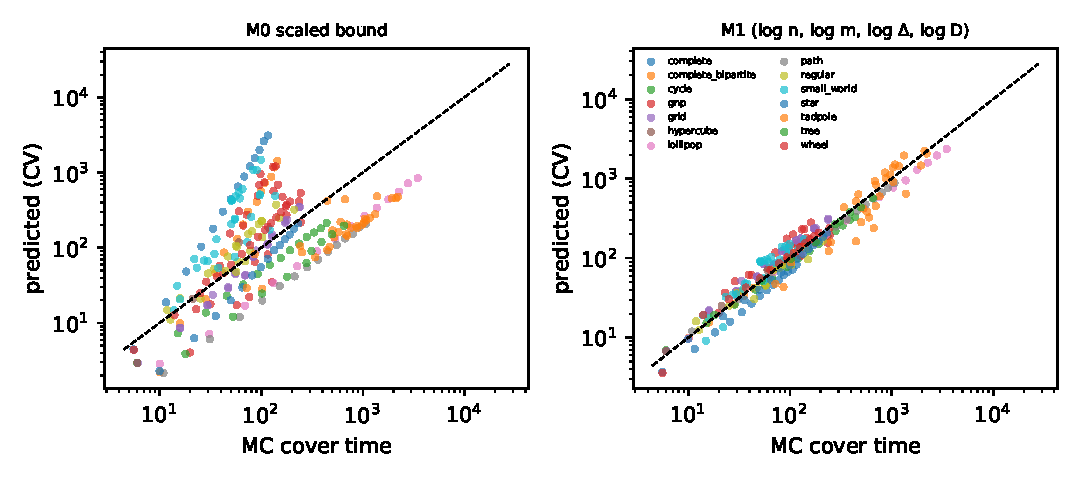
\includegraphics[width=\columnwidth]{fig_pred.pdf}
\end{center}
\caption{Cross-validated predictions against Monte Carlo cover times (log–log), colored by family. Left: rescaled bound (M0). Right: M1. The dashed line is perfect prediction.}
\label{fig:pred}
\end{figure}

\section{Discussion and Limitations}
\label{sec:disc}
\textbf{Answer to the research question.} Yes, for these graphs a four-statistic log-linear model predicts cover time far more accurately than the rescaled $2m(n-1)$ bound: median error about 22\% versus about 150\%. Its reliability depends on the family. It is good when the held-out graph resembles the training families (trees, wheels, bipartite graphs, cycles) and poor for families whose cover time depends on structure that $n$, $m$, $\Delta$ and $D$ do not capture (complete graphs, small-world graphs, and to a lesser extent $G(n,p)$ graphs and stars).

\textbf{Limitations.} (1) The sample is a set of structured families and 247 graphs, not a uniform sample over graphs on $\le 30$ vertices; the fitted coefficients and error rates depend on this mix. (2) The target is the maximum over starts of a Monte Carlo mean, which is slightly biased upward; the effect is small at the measured standard errors. (3) The four features are correlated, so individual coefficients are unstable, and only prediction accuracy is claimed. (4) We do not give a theoretical justification for the log-linear form, and it is not expected to extrapolate beyond $n=30$. (5) We did not compare against other simple baselines (for example, $n$ alone or the Matthews bound) and did not test the predictor on exact cover times; both would be useful next steps. (6) The study used one master seed for the graph generator and one for the simulations; we did not vary it.

\section{Reproducibility}
\label{sec:repro}
Environment: Python 3.11 with numpy, pandas, networkx and matplotlib; gcc for the simulator. Commands (from \texttt{code/}):
\begin{verbatim}
gcc -O2 -o cover cover.c -lm
python run_experiments.py 5000 0   # writes ../results/data.csv (~30 s on 40 cores)
python analyze.py                  # writes ../results/summary.json, family_table.md, fig_pred.pdf
\end{verbatim}
Random seeds: graph generator master seed 0; simulator seed $100000\cdot 0+i+1$ for the $i$-th graph (0-based); bootstrap and CV randomness from \texttt{numpy.random.default_rng(12345)}.

\bibliography{refs}
\bibliographystyle{icml2026}

\end{document}
